\documentclass[journal,12pt,onecolumn]{IEEEtran}
\usepackage{cite}
\usepackage{graphicx}
\usepackage{amsmath,amssymb,amsfonts,amsthm}
\usepackage{algorithmic}
\usepackage{graphicx}
\usepackage{textcomp}
\usepackage{xcolor}
\usepackage{txfonts}
\usepackage{listings}
\usepackage{enumitem}
\usepackage{mathtools}
\usepackage{gensymb}
\usepackage{comment}
\usepackage[breaklinks=true]{hyperref}
\usepackage{tkz-euclide} 
\usepackage{listings}
\usepackage{gvv}                                        
\usepackage[latin1]{inputenc} 
\usetikzlibrary{arrows.meta, positioning}
\usepackage{xparse}
\usepackage{color}                                            
\usepackage{array}                                            
\usepackage{longtable}                                       
\usepackage{calc}                                             
\usepackage{multirow}
\usepackage{multicol}
\usepackage{hhline}                                           
\usepackage{ifthen}                                           
\usepackage{lscape}
\usepackage{tabularx}
\usepackage{array}
\usepackage{float}
\newtheorem{theorem}{Theorem}[section]
\newtheorem{problem}{Problem}
\newtheorem{proposition}{Proposition}[section]
\newtheorem{lemma}{Lemma}[section]
\newtheorem{corollary}[theorem]{Corollary}
\newtheorem{example}{Example}[section]
\newtheorem{definition}[problem]{Definition}
\newcommand{\BEQA}{\begin{eqnarray}}
\newcommand{\EEQA}{\end{eqnarray}}
\usepackage{float}
\theoremstyle{remark}
\usepackage{circuitikz}
\usepackage{tikz}

\title{GG: GEOLOGY AND GEOPHYSICS}
\author{EE25BTECH11032- KARTIK LAHOTI}

\begin{document}

\maketitle 
\begin{enumerate}


    \item Which one of the following is a continental hotspot? \hfill{\brak{\text{GATE GG 2017}}}
        \begin{enumerate} 
            \begin{multicols}{4}
                \item Reunion
                \item Macdonald
                \item Hawaii
                \item Afar
            \end{multicols}
        \end{enumerate}    
    
    \item The diagram given below shows a Mohr circle for two-dimensional stress with points numbered as shown. The mean stress and the maximum shear stress are given by which one of the following number pairs? \hfill{\brak{\text{GATE GG 2017}}}
        \begin{figure}[h]
            \centering
            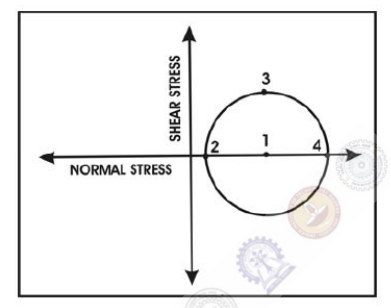
\includegraphics[width=0.3\columnwidth]{Figs/fig_1.png}
            \caption{Q.2.}
            \label{fig:placeholder_1}
        \end{figure}
    
        \begin{enumerate} 
            \item $1\,, 2$
            \item $1\,, 3$
            \item $1\,, 4$
            \item $2\,, 3$
        \end{enumerate}    
    
    \item Which type of fault is developed in the setting shown in the figure below? Velocity vectors on either side of the fault are given in the figure. \hfill{\brak{\text{GATE GG 2017}}}
        \begin{figure}[h]
            \centering
            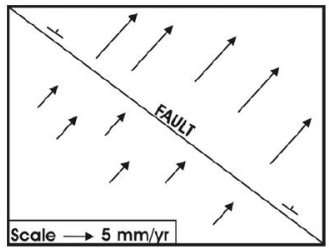
\includegraphics[width=0.5\columnwidth]{Figs/fig_2.png}
            \caption{Q.3.}
            \label{fig:placeholder_2}
        \end{figure}
        \begin{enumerate} 
            \begin{multicols}{2}
                \item Normal
                \item Dextral strike-slip
                \item Sinistral strike-slip
                \item Thrust
            \end{multicols}
        \end{enumerate}    
    
    \item The age of most of the bituminous coal seams of India is \hfill{\brak{\text{GATE GG 2017}}}
        \begin{enumerate} 
            \begin{multicols}{4}
                \item Silurian.
                \item Miocene.
                \item Carboniferous.
                \item Permian.
            \end{multicols}
        \end{enumerate}
        
    \item The time equivalent of the time-stratigraphic term 'Series' is \hfill{\brak{\text{GATE GG 2017}}}
        \begin{enumerate} 
                \item Epoch.
                \item Period.
                \item Age.
                \item Stage.
        \end{enumerate}    
    
    \item Match the following stratigraphic units of India \brak{\text{Group-$I$}} with their age \brak{\text{Group-$II$}}. \hfill{\brak{\text{GATE GG 2017}}}
        \begin{multicols}{2}
            \underline{\textbf{Group $I$}}
            \begin{enumerate}[start=16]
                \item Barakar Formation
                \item Warkalli \brak{\text{Varkala}} Formation
                \item Bagh Beds
                \item Bhander Limestone
            \end{enumerate}
            
            \columnbreak
            
            \underline{\textbf{Group $II$}}
            \begin{enumerate}
                \item Miocene
                \item Cretaceous
                \item Proterozoic
                \item Eocene
                \item Permian
            \end{enumerate}
        \end{multicols}
        \begin{enumerate} 
            \begin{multicols}{2}
                \item P-$5$, Q-$1$, R-$2$, S-$3$
                \item P-$1$, Q-$4$, R-$2$, S-$5$
                \item P-$5$, Q-$4$, R-$2$, S-$3$
                \item P-$2$, Q-$3$, R-$1$, S-$4$
            \end{multicols}        
        \end{enumerate}    
    
    \item Universal Transverse Mercator \brak{\text{UTM}} is a type of \hfill{\brak{\text{GATE GG 2017}}}
        \begin{enumerate} 
            \begin{multicols}{2}
                \item conical projection.
                \item gnomonic projection.
                \item orthogonal projection.
                \item cylindrical projection.
            \end{multicols}
        \end{enumerate}    
    
    \item The groundwater flow equation $\frac{\partial^{2}h}{\partial x^{2}}+\frac{\partial^{2}h}{\partial y^{2}}+\frac{\partial^{2}h}{\partial z^{2}}=0$, where $h$ refers to the hydraulic head and $x$, $y$, $z$ are coordinates, is valid when the flow condition is \hfill{\brak{\text{GATE GG 2017}}}
        \begin{enumerate} 
            \item steady state in isotropic media.
            \item unsteady state in isotropic media.
            \item steady state in anisotropic media.
            \item unsteady state in anisotropic media.
        \end{enumerate}    
    
    \item Los Angeles abrasion test was conducted for a granite aggregate with an initial weight of $4800\text{ grams}$. After the test, the aggregate weighed $3504\text{ grams}$. The Los Angeles abrasion value is \rule{3cm}{0.15mm} $\%$. \hfill{\brak{\text{GATE GG 2017}}}    
    
    \item Brightness temperature is a function of surface temperature and \hfill{\brak{\text{GATE GG 2017}}}
        \begin{enumerate} 
            \begin{multicols}{2}
                \item transmittance.
                \item reflectance.
                \item refractive index.
                \item emissivity.
            \end{multicols}
        \end{enumerate}    
    
    \item Which one of the following minerals has poor cleavage in all directions? \hfill{\brak{\text{GATE GG 2017}}}
        \begin{enumerate} 
            \begin{multicols}{4}
                \item Fluorite
                \item Orthoclase
                \item Quartz
                \item Muscovite
            \end{multicols}
        \end{enumerate}
        
    \item The figure below shows the intercepts of the plane HKL with the crystallographic axes a, b, c. The Miller index of the plane HKL is \hfill{\brak{\text{GATE GG 2017}}}
        \begin{figure}[h]
            \centering
            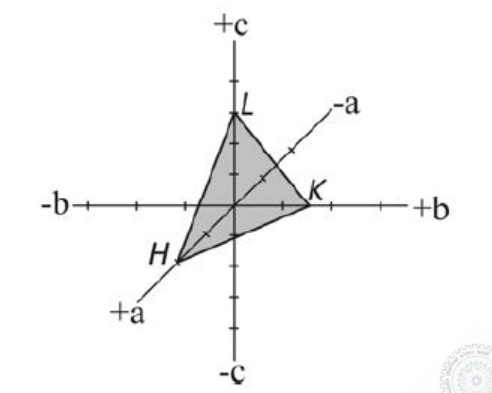
\includegraphics[width=0.5\columnwidth]{Figs/fig_3.png}
            \caption{Q.12.}
            \label{fig:placeholder_3}
        \end{figure}
        \begin{enumerate} 
            \begin{multicols}{4}
                \item $\brak{243}$
                \item $\brak{342}$
                \item $\brak{436}$
                \item $\brak{634}$
            \end{multicols}
        \end{enumerate}    
    
    \item Match the rocks listed in Group-$I$ with the corresponding general rock classification listed in Group-$II$. \hfill{\brak{\text{GATE GG 2017}}}
        \begin{multicols}{2}
            \underline{\textbf{Group $I$}}
            \begin{enumerate}[start=16]
                \item Granite
                \item Basalt
                \item Gneiss
                \item Sandstone
            \end{enumerate}
            
            \columnbreak
            
            \underline{\textbf{Group $II$}}
            \begin{enumerate}
                \item Extrusive igneous rock
                \item Biochemical sedimentary rock
                \item Intrusive igneous rock
                \item Metamorphic rock
                \item Clastic sedimentary rock
            \end{enumerate}
        \end{multicols}
        \begin{enumerate} 
            \begin{multicols}{2}
                \item P-$1$; Q-$3$; R-$5$; S-$2$
                \item P-$4$; Q-$5$; R-$1$; S-$2$
                \item P-$3$; Q-$1$; R-$4$; S-$5$
                \item P-$3$; Q-$4$; R-$1$; S-$5$
            \end{multicols}        
        \end{enumerate}
        
    \item Which one of the following oceanic ridges is known to be aseismic? \hfill{\brak{\text{GATE GG 2017}}}
        \begin{enumerate} 
            \begin{multicols}{2}
                \item Carlsberg
                \item Mid Atlantic
                \item Ninety East
                \item Southwest Indian
            \end{multicols}
        \end{enumerate}
        
    \item Isogonic lines are contours of equal magnetic \hfill{\brak{\text{GATE GG 2017}}}
        \begin{enumerate} 
            \item inclination.
            \item declination.
            \item total field intensity.
            \item horizontal field intensity.
        \end{enumerate}
    \newpage
    \item Match the geophysical terms in Group-$I$ with their corresponding units of measurements in Group-$II$. \hfill{\brak{\text{GATE GG 2017}}}
        \begin{multicols}{2}
            \underline{\textbf{Group $I$}}
            \begin{enumerate}[start=16]
                \item Transit time
                \item Conductivity
                \item Gravity anomaly
                \item Magnetic field intensity
            \end{enumerate}
            
            \columnbreak
            
            \underline{\textbf{Group $II$}}
            \begin{enumerate}
                \item mGal
                \item nanoTesla
                \item siemens
                \item millivolt
                \item microsecond per feet
            \end{enumerate}
        \end{multicols}
        \begin{enumerate} 
            \begin{multicols}{2}     
                \item P-$5$; Q-$4$; R-$2$; S-$1$
                \item P-$5$; Q-$4$; R-$3$; S-$2$
                \item P-$5$; Q-$3$; R-$1$; S-$2$
                \item P-$4$; Q-$3$; R-$2$; S-$1$
            \end{multicols}        
        \end{enumerate}
        
    \item The Maxwell's equation based on Ampere's law is \hfill{\brak{\text{GATE GG 2017}}}
        \begin{enumerate} 
                \item $\nabla\times E=-\frac{\partial B}{\partial t}$ 
                \item $\nabla\times H=j+\frac{\partial D}{\partial t}$ 
                \item $\nabla\cdot B=0$ 
                \item $\nabla\cdot E=\frac{\rho}{\epsilon}$ 
        \end{enumerate}
        
    \item The normal gravity formula $\brak{\text{for e.g. GRS}80}$ is a function of \hfill{\brak{\text{GATE GG 2017}}}
        \begin{enumerate} 
                \item geocentric latitude.
                \item geodetic latitude.
                \item longitude.
                \item altitude.
        \end{enumerate}
    
    \item A seismic reflection survey was carried out over a subsurface consisting of a stack of horizontal isotropic layers. In the common midpoint \brak{\text{CMP}} domain, the moveout \brak{\text{traveltime v/s offset}} curve for any primary reflection event is best approximated by \hfill{\brak{\text{GATE GG 2017}}}
        \begin{enumerate} 
                \item an ellipse.
                \item a parabola.
                \item a circle.
                \item a hyperbola.
        \end{enumerate}
        
    \item Assertion \brak{\text{a}}: Magnetic stripes are observed around mid-oceanic ridge regions.
    
    Reason \brak{\text{r}}: The earth's magnetic field undergoes reversals of polarity. \hfill{\brak{\text{GATE GG 2017}}}
        \begin{enumerate} 
            \item \brak{\text{a}} is true but \brak{\text{r}} is false.
            \item \brak{\text{a}} is false but \brak{\text{r}} is true.
            \item Both \brak{\text{a}} and \brak{\text{r}} are true and \brak{\text{r}} is one of the correct reasons for (a).
            \item Both \brak{\text{a}} and \brak{\text{r}} are true but \brak{\text{r}} is not the correct reason for \brak{\text{a}}.
        \end{enumerate}
    
    \item A seismic gap refers to a \hfill{\brak{\text{GATE GG 2017}}}
        \begin{enumerate} 
            \item time gap between two great earthquakes.
            \item distance gap between the epicenters of two great earthquakes.
            \item segment of an active belt where a historical great earthquake has not occurred.
            \item wide gap in the earth created by a great earthquake.
        \end{enumerate}
    
    \item The travel time difference between the arrival times of a shear wave $\brak{S}$ and primary wave $\brak{P}$ observed on a seismogram recorded at an epicentral distance of $100\,km$ from a near surface earthquake is \rule{3cm}{0.15mm}s. (Assume the average $P$ and $S$ wave velocities to be $6.0\,km/s $ and $3.5\,km/s $, respectively). \hfill{\brak{\text{GATE GG 2017}}}
    
    \item The percentage increase in P-wave velocity $\brak{km/s}$ across the Mohorovicic discontinuity from the lower crust to the upper mantle beneath a craton is approximately \rule{3cm}{0.15mm} $\brak{\%}$. \hfill{\brak{\text{GATE GG 2017}}}
    
    \item Which one amongst the following logging tools has the largest depth of investigation? \hfill{\brak{\text{GATE GG 2017}}}
        \begin{enumerate} 
            \begin{multicols}{4}
                \item Density
                \item Laterolog $3$
                \item Laterolog $8$
                \item Neutron
            \end{multicols}
        \end{enumerate}
    
    \item The most abundant radioactive isotope in the continental crust is \hfill{\brak{\text{GATE GG 2017}}}
        \begin{enumerate} 
            \begin{multicols}{4}
                \item $^{40}K$ 
                \item $^{232}Th$ 
                \item $^{235}U$ 
                \item $^{238}U$ 
            \end{multicols}
        \end{enumerate}
    
    \section*{Geology \brak{\text{Part B}} \brak{\text{Section-1}}}
    
    \item Stylolitic foliation developed during diagenetic processes is typically \hfill{\brak{\text{GATE GG 2017}}}
        \begin{enumerate} 
            \item parallel to bedding.
            \item perpendicular to bedding.
            \item oblique to bedding.
            \item vertical.
        \end{enumerate}
    
    \item A coal seam with an attitude $090\degree \,,50\degree S$ outcrops at an elevation of $1400\,m$ in an area that has flat topography. A vertical exploratory drill hole will intersect the seam \hfill{\brak{\text{GATE GG 2017}}}
        \begin{enumerate} 
            \item north of the outcrop at elevations greater than $1400\,m$.
            \item north of the outcrop at elevations less than $1400\,m$.
            \item south of the outcrop at elevations less than $1400\,m$.
            \item south of the outcrop at elevations greater than $1400\,m$.
        \end{enumerate}
    
    \item Earthquakes result in the formation of which one of the following features? \hfill{\brak{\text{GATE GG 2017}}}
        \begin{enumerate} 
            \begin{multicols}{4}
                \item Porphyroblast
                \item Porphyroclast
                \item Pseudotachylite
                \item Pressure shadow
            \end{multicols}
        \end{enumerate}
    
    \item In a bilaterally symmetrical brachiopod fossil, the angle between the hinge line and the median line changes to $45\degree$ after deformation. The shear strain observed in the deformed fossil is \rule{3cm}{0.15mm}. \hfill{\brak{\text{GATE GG 2017}}}
    
    \item The empirical probability distribution of gold $\brak{Au}$ grades shows a unimodal distribution with mode $=2\,g/t$, median $=3\,g/t$, and mean $=5\,g/t$. This probability distribution is \hfill{\brak{\text{GATE GG 2017}}}
        \begin{enumerate} 
            \item positively skewed.
            \item negatively skewed.
            \item normally distributed.
            \item platykurtic.
        \end{enumerate}
    
    \item A limb of a non-plunging fold with an attitude $070\degree\, , 40\degree S$ is rotated about its fold axis $30\degree$ clockwise \brak{\text{looking towards ENE}}. The plunge amount of the pole to the fold limb after rotation is \rule{3cm}{0.15mm} degrees. \hfill{\brak{\text{GATE GG 2017}}}
    
    \item The Bulk Silicate Earth \brak{\text{BSE}} is best approximated by the average \hfill{\brak{\text{GATE GG 2017}}}
        \begin{enumerate} 
            \item enriched upper mantle composition.
            \item mantle and continental crust composition.
            \item depleted mantle composition.
            \item primitive upper mantle composition.
        \end{enumerate}
    
    \item Which one of the following is the stable mineral assemblage in metamorphism of a rock with pelitic bulk composition under granulite facies? \hfill{\brak{\text{GATE GG 2017}}}
        \begin{enumerate} 
            \item staurolite $+$ muscovite $+$ sillimanite $+$ K-feldspar 
            \item phengite $+$ garnet $+$ chloritoid $+$ biotite 
            \item garnet $+$ orthopyroxene $+$ clinopyroxene $+$ plagioclase 
            \item garnet $+$ cordierite $+$ K-feldspar $+$ sillimanite 
        \end{enumerate}
        
    \item The given P-T diagram shows four distinct metamorphic paths designated as $1$, $2$, $3$ and $4$. Which one of these P-T paths represents crustal thickening in a collisional tectonic setting? \hfill{\brak{\text{GATE GG 2017}}}
        \begin{figure}[h]
            \centering
            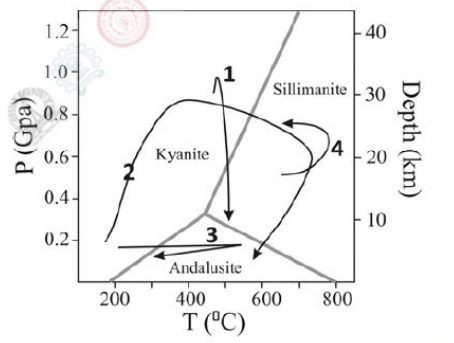
\includegraphics[width=0.5\columnwidth]{Figs/fig_4.png}
            \caption{Q.34.}
            \label{fig:placeholder_4}
        \end{figure}
        \begin{enumerate} 
            \begin{multicols}{4}
                \item $1$
                \item $2$
                \item $3$
                \item $4$
            \end{multicols}
        \end{enumerate}
    
    \item The pressure on a rock overlain by a $7\,km$ thick basaltic crust ($\rho=3100\,kg\,m^{-3}$) is \rule{3cm}{0.15mm} kilobar. (Use $g=9.8\,ms^{-2}$; $10^5\,Pa=1 bar$) \hfill{\brak{\text{GATE GG 2017}}}
    
    \item The given T-X diagram shows the phase relations in olivine solid solution at $1$ bar pressure. If '$P$' is the initial position of melt, the proportion of melt at $1500\degree$C is \rule{3cm}{0.15mm}$\%$. \hfill{\brak{\text{GATE GG 2017}}}
        \begin{figure}[h]
            \centering
            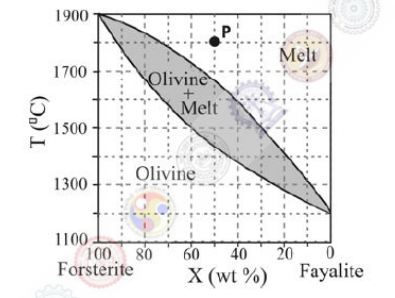
\includegraphics[width=0.5\columnwidth]{Figs/fig_5.png}
            \caption{Q.36.}
            \label{fig:placeholder_5}
        \end{figure}
    
    \item Fluorite crystal $\brak{CaF_2}$ adopts face-centered cubic structure with lattice parameter $a=5.463$ \AA. If the ionic radius of anion $\brak{F^{-}}$ is $1.31$ \AA, the ionic radius of cation $\brak{Ca^{2+}}$ is \rule{3cm}{0.15mm} \AA. \hfill{\brak{\text{GATE GG 2017}}}
    
    \item The diagram below shows the interference figure of a mineral. The mineral is \hfill{\brak{\text{GATE GG 2017}}}
        \begin{figure}[h]
            \centering
            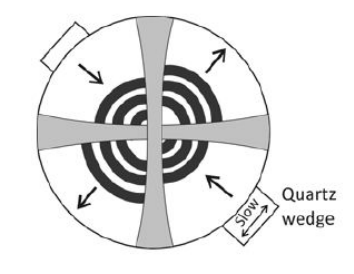
\includegraphics[width=0.5\columnwidth]{Figs/fig_6.png}
            \caption{Q.38.}
            \label{fig:placeholder_6}
        \end{figure}
        \begin{enumerate} 
            \item uniaxial positive
            \item biaxial negative
            \item uniaxial negative
            \item biaxial positive
        \end{enumerate}
    
    \item The standard thermodynamic data for enstatite $\brak{Mg_2Si_2O_6}$, quartz $\brak{SiO_2}$ and forsterite $\brak{Mg_2SiO_4}$ is given in the table below. The Gibbs' free energy of the reaction $\brak{Mg_2Si_2O_6 + SiO_2 = Mg_2SiO_4}$ at $600\,K$ and $1\,bar$ is \rule{3cm}{0.15mm} $J$. (Assume $C_p=0$ for all minerals in the reaction) \hfill{\brak{\text{GATE GG 2017}}}
        \begin{table}[H]
            \centering
            \begin{center}
\begin{tabular}{ll}
    \textbf{Group I} & \textbf{Group II} \\
    P. Ferrite & 1. Hexagonal Close Packed (HCP) \\
    Q. Austenite & 2. Body Centered Cubic (BCC) \\
    R. Martensite & 3. Body Centered Tetragonal (BCT) \\
    & 4. Face Centered Cubic (FCC)
\end{tabular}
\end{center}   
        \end{table}
    
    \item The modal abundance in an ultramafic rock and the partition coefficients of lutetium $\brak{Lu}$ in clinopyroxene, orthopyroxene, olivine and plagioclase are tabulated below. The bulk distribution coefficient of lutetium $\brak{D_{Lu})}$ in the ultramafic rock is \rule{3cm}{0.15mm}. \hfill{\brak{\text{GATE GG 2017}}}
        \begin{table}[H]
            \centering
            \begin{tabular}{|c|c|c|}
     \hline
     \textbf{Mineral} & \textbf{Modal abundance \brak{\%}} & \textbf{Partition coefficient}\\
     \hline
     Clinopyroxene & $45$ & $0.506$ \\
      \hline
      Orthopyroxene & $40$ & $0.42$ \\
      \hline
      Olivine & $10$ & $0.045$ \\
      \hline
      Plagioclase & $05$ & $0.019$ \\
      \hline
\end{tabular}
        \end{table}
    
    \item Match the following classical ore deposits (Group-$I$) with their associated ore minerals (Group-$II$). \hfill{\brak{\text{GATE GG 2017}}}
        \begin{multicols}{2}
            \underline{\textbf{Group $I$}}
            \begin{enumerate}[start=16]
                \item Sudbury type deposit
                \item Mississippi valley type deposit
                \item Climax type deposit
                \item IOCG type deposit
            \end{enumerate}
            
            \columnbreak
            
            \underline{\textbf{Group $II$}}
            \begin{enumerate}
                \item Molybdenite
                \item Uraninite and chalcopyrite
                \item Pentlandite
                \item Psilomelane
                \item Sphalerite and Galena
            \end{enumerate}
        \end{multicols}
        \begin{enumerate}
            \begin{multicols}{2}  
            \item P-$4$; Q-$5$; R-$2$; S-$1$
            \item P-$3$; Q-$5$; R-$1$; S-$2$
            \item P-$5$; Q-$2$; R-$4$; S-$1$
            \item P-$3$; Q-$5$; R-$2$; S-$4$
            \end{multicols}        
        \end{enumerate}
    
    \item Which one of the following microfossils is commonly used in biostratigraphic correlation of Palaeozoic marine strata? \hfill{\brak{\text{GATE GG 2017}}}
        \begin{enumerate} 
            \begin{multicols}{4}
                \item Angiosperm pollen
                \item Diatoms
                \item Dinoflagellates
                \item Chitinozoans
            \end{multicols}
        \end{enumerate}
    
    \item Given below are pairs of "living fossils". Which one of the following is a brachiopod-mollusc pair? \hfill{\brak{\text{GATE GG 2017}}}
        \begin{enumerate} 
            \item \textit{Lingula, Nautilus}
            \item \textit{Ginkgo, Metasequoia}
            \item \textit{Sphenodon, Notorhynchus}
            \item Coelacanths, \textit{Sidderoidea}
        \end{enumerate}
    
    \item Match the sedimentary rocks and their features listed in Group $I$ with depositional environments listed in Group $II$. \hfill{\brak{\text{GATE GG 2017}}}
        \begin{multicols}{2}
            \underline{\textbf{Group $I$}}
            \begin{enumerate}[start=16]
                \item Sandstone with herring-bone cross bedding
                \item Chalk with coccolith
                \item Well sorted arenite with large cross bedding (5-10 m thick)
                \item Poorly sorted sediments with faceted and striated pebbles
            \end{enumerate}
            
            \columnbreak
            
            \underline{\textbf{Group $II$}}
            \begin{enumerate}
                \item Eolian
                \item Glacial
                \item Sabkha
                \item Tidal
                \item Pelagic
            \end{enumerate}
        \end{multicols}
        \begin{enumerate} 
            \begin{multicols}{2}  
                \item P-$2$, Q-$1$, R-$4$, S-$5$
                \item P-$4$, Q-$5$, R-$1$, S-$2$
                \item P-$4$, Q-$1$, R-$2$, S-$5$
                \item P-$5$, Q-$1$, R-$2$, S-$3$
            \end{multicols}        
        \end{enumerate}
    
    \item Arrange the following stratigraphic formations sequentially from older to younger: (P) Jodhpur Sandstone (Q) Cambay Shale (R) Krol Limestone (S) Tipam Sandstone \hfill{\brak{\text{GATE GG 2017}}}
        \begin{enumerate} 
            \begin{multicols}{2}
                \item P, R, Q, S
                \item R, Q, P, S
                \item P, S, R, Q
                \item R, P, Q, S
            \end{multicols}
        \end{enumerate}
    
    \item $2\,g$ air dried coal contains $0.2\,g$ moisture, $0.3\,g$ ash and $0.5\,g$ volatile matter. The volatile matter content in the coal in dry mineral matter free \brak{d.m.f} basis is \rule{3cm}{0.15mm} $\%$. (mineral matter content $=1.1 \times$ ash content) \hfill{\brak{\text{GATE GG 2017}}}
    
    \item The approximate temperature for "oil window" ranges from \hfill{\brak{\text{GATE GG 2017}}}
        \begin{enumerate} 
            \begin{multicols}{2}
                \item $30\degree C \text{ to } 50\degree C$
                \item $60\degree C \text{ to } 160\degree C$
                \item $180\degree C \text{ to } 250\degree C$
                \item $260\degree C \text{ to } 350\degree C$
            \end{multicols}
        \end{enumerate}
    
    \item Which one of the following biopolymers is the major source of liquid hydrocarbons? \hfill{\brak{\text{GATE GG 2017}}}
        \begin{enumerate} 
            \item Lignin
            \item Proteins
            \item Lipids
            \item Carbohydrates
        \end{enumerate}
    
    \item The hydraulic conductivity $\brak{K}$ of an isotropic aquifer is $10\, m/day$. If the hydraulic head within the aquifer drops $4\,m$ over a distance of $750\,m$ , the groundwater flow velocity within the aquifer is \rule{3cm}{0.15mm}$m/day$. (Up to third decimal place) \hfill{\brak{\text{GATE GG 2017}}}
    \newpage
    \item Drainage network of a watershed ordered as per the Strahler method is given below. Maximum observed bifurcation ratio for the given network is \rule{3cm}{0.15mm}. \hfill{\brak{\text{GATE GG 2017}}}
        \begin{figure}[h]
            \centering
            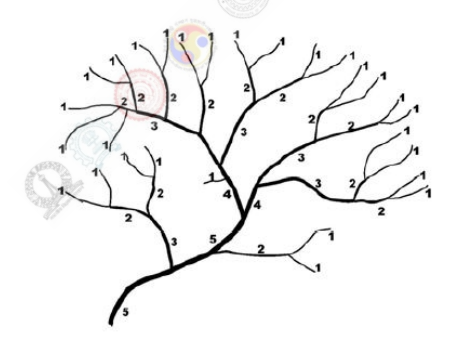
\includegraphics[width=0.5\columnwidth]{Figs/fig_7.png}
            \caption{Q.50.}
            \label{fig:placeholder_7}
        \end{figure}
    
    \item In a vertical aerial photo, the top and bottom of a tower built on a flat terrain is displaced by $2\,mm$. In the photograph, the distance between top of the tower and nadir point is $100\,mm$ . The flying height of the aircraft was $3000\,m$  above the ground. The estimated height of the tower is \rule{3cm}{0.15mm} $m$. \hfill{\brak{\text{GATE GG 2017}}}
    
    \item Brazilian test was conducted on a rock sample having radius of $27\,mm$  and thickness of $22\, mm$ . The failure load was $5\,kN$ . The tensile strength of the rock is \rule{3cm}{0.15mm} $N/mm^{2}$. \hfill{\brak{\text{GATE GG 2017}}}
    
    \item The average assay \brak{\text{a}} and area of influence \brak{\text{A}} of a placer gold deposit of uniform thickness sampled at four locations W, X, Y and Z are given below. The weighted average assay of the ore body is \rule{3cm}{0.15mm} $g/t$. \hfill{\brak{\text{GATE GG 2017}}}
        \begin{figure}[h]
            \centering
            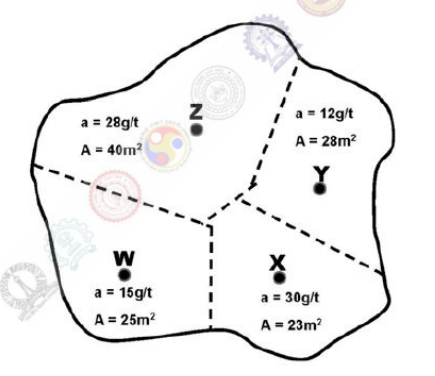
\includegraphics[width=0.5\columnwidth]{Figs/fig_8.png}
            \caption{Q.53.}
            \label{fig:placeholder_8}
        \end{figure}
    
    \item The minimum and maximum values of the digital number \brak{\text{DN}} of a remote sensing image are $8$ and $32$ respectively. The digital data was linearly stretched between $0$ and $255$ by using min-max linear stretching method. The post stretched integer DN value of a pixel with an original DN value of $27$ will be \rule{3cm}{0.15mm}. \hfill{\brak{\text{GATE GG 2017}}}
    
    \item The length and width of concave and convex sides of a landslide is shown in the figure below. The Dilation Index of the landslide is \rule{3cm}{0.15mm}. \hfill{\brak{\text{GATE GG 2017}}}
    
        \begin{figure}[h]
            \centering
            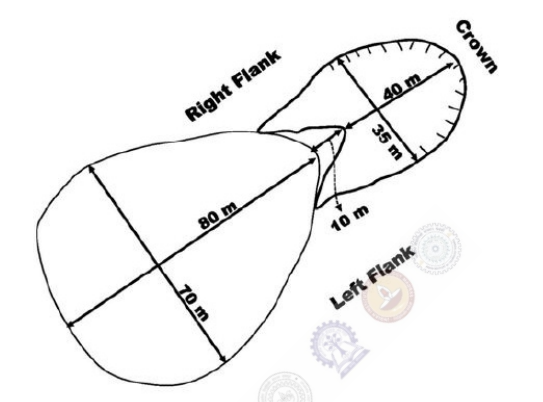
\includegraphics[width=0.5\columnwidth]{Figs/fig_9.png}
            \caption{Q.55.}
            \label{fig:placeholder_9}
        \end{figure}
    
    \section*{Geophysics \brak{Part B} \brak{Section-2}}
    
    \item Which one of the following seismic phases is observable in the P-wave shadow zone? \hfill{\brak{\text{GATE GG 2017}}}
        \begin{enumerate} 
            \begin{multicols}{4}
                \item P
                \item PnP
                \item PcS
                \item PKIKP
            \end{multicols}
        \end{enumerate}
    
    \item Consider a geological body buried at the equator at a certain depth. If the same body were to be buried at the North pole at the same depth, how would the gravity and magnetic field responses measured over the body differ? Assume the same magnetic susceptibility and density contrasts. \brak{\text{Consider only geomagnetic induction}} \hfill{\brak{\text{GATE GG 2017}}}
        \begin{enumerate} 
            \item Both gravity and magnetic field responses do not change
            \item Both gravity and magnetic field responses change significantly
            \item Gravity field response changes significantly but magnetic field response does not change
            \item Gravity field response does not change but magnetic field response changes significantly
        \end{enumerate}
    
    \item Given the Bouguer density of $2.8\,g/cc$, the Bouguer correction for a gravity station at an elevation of $30\,m$ above the datum is \rule{3cm}{0.15mm} $mGals$. $\brak{\text{Use } \pi=3.14}$ \hfill{\brak{\text{GATE GG 2017}}}
    
    \item Given the following data for a resistivity sounding experiment over a two-layered half-space, the resistivity transform for the top layer is \rule{3cm}{0.15mm} $\Omega m$. (Data: resistivity of top layer $\rho_1=10\,\Omega m$, resistivity of half space $\rho_2=100\,\Omega m$, thickness of top layer $h_1=10\,m$ and current electrode spacing $AB/2 = 5\,m$ ) \hfill{\brak{\text{GATE GG 2017}}}
    
    \item The ratio of eccentricity to the polar flattening of an ellipsoidal Earth with equatorial radius '$a$' and polar radius '$b$' can be expressed as \hfill{\brak{\text{GATE GG 2017}}}
        \begin{enumerate} 
            \begin{multicols}{4}
                \item $\frac{\sqrt{e^2+p^2}}{\sqrt{e-p}}$
                \item $\frac{\sqrt{e^2-p^2}}{\sqrt{e+p}}$
                \item $\frac{\sqrt{e+p}}{\sqrt{e-p}}$
                \item $\frac{\sqrt{e^2+p^2}}{\sqrt{e+p}}$
            \end{multicols}
        \end{enumerate}
    
    \item The vertical field intensity anomaly $A_z$ due to a vertically polarized vertical dyke is given by $$ A_z = 2Mt\brak{\frac{z_1}{\brak{z_1^2+x^2}} - \frac{z_2}{\brak{z_2^2+x^2}}}$$ where $M$ is the magnitude of intensity of magnetization. All relevant parameters are provided in the figure below. The dyke has $1\%$ magnetite (magnetic susceptibility of magnetite = $0.5$ SI unit) distributed homogeneously. Then, the magnitude of peak vertical field intensity over the dyke is \rule{3cm}{0.15mm} $nT$.  \hfill{\brak{\text{GATE GG 2017}}}
    
    \begin{figure}[H]
        \centering
        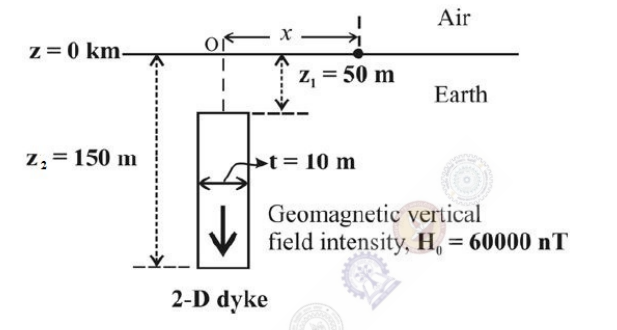
\includegraphics[width=0.5\columnwidth]{Figs/fig_10.png}
        \caption{Q.61.}
        \label{fig:placeholder_10}
    \end{figure}
    
    \item In a magneto-telluric (MT) experiment over a homogeneous and isotropic half-space, the apparent resistivity is $50\,\Omega m$ for an electric field intensity of $12\,mV/km$ and time period of $10\,s$. Then, the magnetic field strength is \rule{3cm}{0.15mm} $nT$. \hfill{\brak{\text{GATE GG 2017}}}
    
    \item The apparent resistivity for Wenner and Schlumberger configurations in an electrical sounding experiment is the same for a certain electrode spacing a (Wenner configuration). Given the current electrode spacing of $18 m$ and the potential electrode spacing of $2 m$ for a Schlumberger configuration, the value of a is \rule{3cm}{0.15mm} $m$. \hfill{\brak{\text{GATE GG 2017}}}
    
    \item In a time-domain (T-D) induced polarization experiment with a steady voltage of $10 mV$ during the current flow interval, the voltage decay after the current cut-off is given by:
    $$v\brak{t} = 4.0e^{-0.3t}mV$$ 
    The chargeability after current cut-off between $t_1 = 1s \text{and} t_2 = 4s $ is \rule{3cm}{0.15mm} $ms$ . \hfill{\brak{\text{GATE GG 2017}}}
    
    \item Which one of the following statements is TRUE for a near-surface earthquake occurring in a homogeneous, isotropic Earth? \hfill{\brak{\text{GATE GG 2017}}}
                \begin{enumerate}
                        \item Rayleigh waves are generated.
                        \item Love waves are generated.
                        \item Shear waves are split. 
                        \item P waves undergo refraction.
                \end{enumerate}
            
    \item A dynamic range of $60 dB$ in power corresponds to an increase in amplitude by a factor of \rule{3cm}{0.15mm}. \hfill{\brak{\text{GATE GG 2017}}}
    
    \item The slope of the Wadati plot obtained using the $P$ and $S$ arrival times of a local earthquake is $1.0$. The corresponding $V_p/V_S$ ratio of the subsurface medium is \rule{3cm}{0.15mm}. \hfill{\brak{\text{GATE GG 2017}}}
    
    \item The beach ball figure given below depicts the focal mechanism of an earthquake. The shaded and unshaded portions indicate compressional and dilatational quadrants, respectively. $FP1$ is the fault plane solution. The focal mechanism and $FP1$ represent: \hfill{\brak{\text{GATE GG 2017}}}
        \begin{figure}[H]
            \centering
            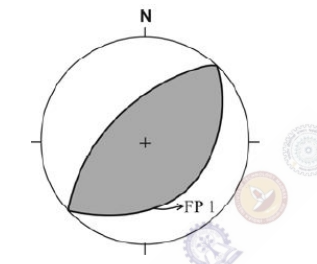
\includegraphics[width=0.5\columnwidth]{Figs/fig_11.png}
            \caption{Q.68.}
            \label{fig:placeholder_}
        \end{figure}
                \begin{enumerate}
                        \item A thrust fault with strike 45\degree and dip 30\degree with the tension axis in the compression quadrant.
                        \item A normal fault with strike $45\degree$ and dip $30\degree$ with the tension axis in the compression quadrant.
                        \item A thrust fault with strike $225\degree$ and dip $60\degree$ with the pressure axis in the compression quadrant.
                        \item A normal fault with strike $225\degree$ and dip $60\degree$ with the pressure axis in the compression quadrant.
                \end{enumerate}
     \item The characteristic log responses of a thick coal seam are: \hfill{\brak{\text{GATE GG 2017}}}
                \begin{enumerate}
                        \item Low transit time, low resistivity and high gamma ray count.
                        \item Low transit time, low resistivity and low gamma ray count.
                        \item High transit time, high resistivity and low gamma ray count.
                        \item High transit time, low resistivity and high gamma ray count.
                \end{enumerate}
    \item The SP response of a thick, clean sandstone bed is $-54 mV$. Given the mud filtrate resistivity to be $0.45\Omega m$  at a formation temperature of $130\degree F$ and the coefficient $K = 77.29$, the formation water resistivity is \rule{3cm}{0.15mm} $\Omega\,m$. \hfill{\brak{\text{GATE GG 2017}}}
    
    \item Which one of the following log responses is TRUE for a porous and permeable sandstone bed, when the resistivity of the mud filtrate used is equal to the resistivity of the formation water?\hfill{\brak{\text{GATE GG 2017}}}
                \begin{enumerate}
                        \item A large negative SP is observed.
                        \item A large positive SP is observed.
                        \item LLs and LLm logs show appreciably large separation.
                        \item LLm and LLd logs overlap with each other.
                \end{enumerate}
    
    \item The number of half-lives $\brak{T_{1/2}}$  required for a certain amount of radioactive isotope in a rock to reduce to $3\%$ of its original amount is \rule{3cm}{0.15mm}\hfill{\brak{\text{GATE GG 2017}}}
    
    \item VLF fields can be measured over continental distances $\brak{r}$ because: \hfill{\brak{\text{GATE GG 2017}}}
                \begin{enumerate}
                        \item The magnetic field decreases at the rate $1/r$ and the output at the transmitting station is $1$ to $10 kW$.
                        \item  The magnetic field decreases at the rate $1/{r^3}$and the output power at the transmitting station is $1$ to $10 kW$.
                        \item The magnetic field decreases at the rate $1/r$and the output power at the transmitting station is $100$ to $1000 kW$.
                        \item The magnetic field decreases at the rate $1/{r^2}$ and the output power at the transmitting station is $100$ to $1000 kW$.
                \end{enumerate}
    
    \item  Convolution of two boxcar functions of different widths yields a: \hfill{\brak{\text{GATE GG 2017}}}
                \begin{enumerate}
                    \begin{multicols}{2}
                        \item Stem function.
                        \item Trapezoidal function.
                        \item Boxcar function.
                        \item Sinc functon.
                    \end{multicols}
                \end{enumerate}
    
    \item Assuming the Z-transform to be defined with $Z$ as the unit delay operator, the pole of the infinite sequence $\sbrak{1,1/2,1/4,1/8,\dots}$ is at $Z = $ \rule{3cm}{0.15mm}. \hfill{\brak{\text{GATE GG 2017}}}
    
    \item Normal moveout (NMO) correction was applied to seismic data in the common midpoint (CMP) domain. The frequency distortion due to NMO stretch is highest for: \hfill{\brak{\text{GATE GG 2017}}}
                \begin{enumerate}
                    \begin{multicols}{2}
                        \item Larger offsets of deeper reflections.
                        \item Smaller offsets of shallower reflections.
                        \item Larger offsets of shallower reflections.
                        \item Smaller offsets of deeper reflections.
                    \end{multicols}
                \end{enumerate}
    
    \item Consider a hypothetical zero-offset seismic reflection survey acquired over a reflector whose dip is $30\degree$. The velocity of the medium above the reflector is $2 km/s$ and the trace spacing is $25 m$. The maximum unaliased frequency in the data is \rule{3cm}{0.15mm} $Hz$. (HInt: The difference in traveltime between adjacent traces should be less than or equal to half a cycle.) \hfill{\brak{\text{GATE GG 2017}}}
    
    \item In statistical wavelet deconvolution, the reflectivity series is assumed to be a random sequence. Then, the autocorrelation of the wavelet is: \hfill{\brak{\text{GATE GG 2017}}}
                \begin{enumerate}
                        \item A scaled version of the autocorrelation of the seismic trace.
                        \item A random sequence.
                        \item Zero.
                        \item  Dirac delta function.
                \end{enumerate}
                
    \item A vector field $u$ is expressed by its Helmholtz decomposition as: 
    $$ u = \nabla\phi + \nabla \times \psi $$ with $\phi = \frac{1}{2}\brak{x^2 - y^2 +z^2} \text{ and } \psi = zy^2i + xzj + x^2k $ The magnitude of the ivergence of the vector field $u$ at $\brak{1,1,1}$ is \rule{3cm}{0.15mm} \hfill{\brak{\text{GATE GG 2017}}}
    
    \item In the figure shown, a ray corresponding to a P-wave is incident on the interface between layer $1$ and layer $2$ at an angle of $30\degree$ The P-wave velocity is $1 km/s$, $1.2 km/s$, and $1.5 km/s$ in layer $1$, layer $2$, and the half-space, respectively. The emergence angle of the ray into the half-space is \rule{3cm}{0.15mm} degrees.  \hfill{\brak{\text{GATE GG 2017}}}
    
    \begin{figure}[h]
        \centering
        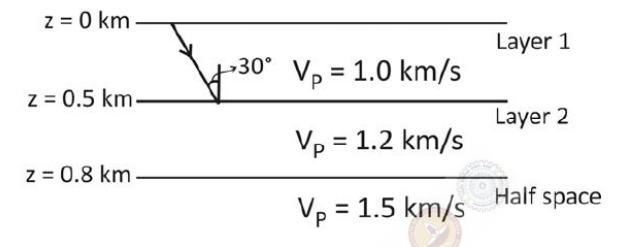
\includegraphics[width=0.5\columnwidth]{Figs/fig_12.png}
        \caption{Q.80.}
        \label{fig:placeholder_12}
    \end{figure}
    
    \item How do the P-wave velocity $\brak{V_p}$ S-wave velocity $\brak{V_s}$, and Poisson's ratio $\brak{\sigma}$ change from a water-saturated sandstone to a gas-saturated sandstone? \hfill{\brak{\text{GATE GG 2017}}}
                \begin{enumerate}
                        \item $\brak{V_p}$ increases, $\brak{V_p}$ decreases, and $\sigma$ increases.
                        \item $\brak{V_p}$ decreases, $\brak{V_s}$ remains the same, and $\sigma$ decreases.
                        \item $\brak{V_p}$ decreases, $\brak{V_s}$ increases, and $\sigma$ decreases.
                        \item $\brak{V_p}$, $\brak{V_p}$, and $\sigma$ all remain constant.
                \end{enumerate}
    
    \item In a VSP experiment, the subsurface consists of a horizontal layer of $2 km$ thickness underlain by a semi-infinite half-space. The P-wave velocities $\brak{V_p}$ in the first layer and half-space are $2.0 km/s$ and $2.5 km/s$, respectively. A vertical well has receivers spaced $10 m$ apart, from depth $0.5 km$ to $1.5 km$. The source is placed $0.5 km$ from the well head.The traveltime of the primary reflection event at the deepest receiver is \rule{3cm}{0.15mm}s. \hfill{\brak{\text{GATE GG 2017}}}
    
    \begin{figure}[h]
        \centering
        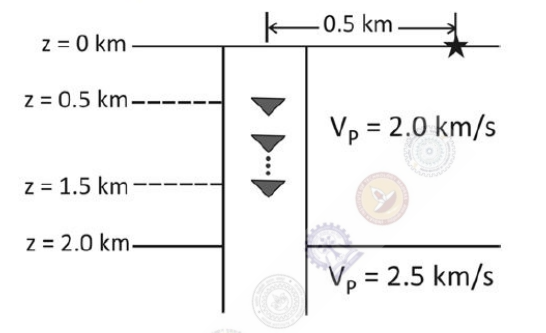
\includegraphics[width=0.5\columnwidth]{Figs/fig_13.png}
        \caption{Q.82.}
        \label{fig:placeholder_13}
    \end{figure}
    
    \item Which one of the following sets of vectors $\cbrak{V_1,V_2,V_3}$ is lineraly dependent?\hfill{\brak{\text{GATE GG 2017}}}
                \begin{enumerate}
                        \item $V_1 = \brak{0,-1,3}, V_2 = (2,0,1), v_3 =(-2,-1,3)$
                        \item $V_1 = \brak{2,-2,0}, V_2 = (0,1,-1), v_3 =(0,4,2)$
                        \item $V_1 = \brak{2,6,2}, V_2 = (2,0,-2), v_3 =(0,4,2)$
                        \item $V_1 = \brak{1,4,7}, V_2 = (2,5,8), v_3 =(3,6,9)$
                \end{enumerate}
    
    \item Thecondition number for the matrix $A = \myvec{2 & 1 \\ 0 & 3}$ is \rule{3cm}{0.15mm}  \hfill{\brak{\text{GATE GG 2017}}}
    
                
    \item Match the items in Group $I$ with their corresponding analytical expressions in Group $II$:  \hfill{\brak{\text{GATE GG 2017}}}
    
            \begin{multicols}{2}
                \underline{\textbf{Group $I$}}
                \begin{enumerate}[start =16]
                    \item Wave equation
                    \item Heat conduction equation
                    \item Eikonal equation
                    \item Poisson equation
                \end{enumerate}
    
                \columnbreak
    
                \underline{\textbf{Group $II$}}
                \begin{enumerate}
                    \item $\mydet{\nabla u}^2 = 1 $
                    \item $\frac{\partial^2u}{\partial t^2} - \nabla^2 u = 0$
                    \item $\nabla^2u = -4\pi\sigma$
                    \item $\frac{\partial u}{\partial t} - \nabla^2u=0$
                    \item $\frac{\partial u}{\partial t} + u\cdot\nabla u = 0 $
                \end{enumerate}
            \end{multicols}
    
            \begin{enumerate}
                \begin{multicols}{2}
                    \item P-$2$, Q-$3$, R-$4$, S-$1$
                    \item P-$2$, Q-$4$, R-$1$, S-$3$
                    \item P-$4$, Q-$2$, R-$5$, S-$3$
                    \item P-$4$, Q-$3$, R-$1$, S-$5$
                \end{multicols}
            \end{enumerate}
    
    \begin{center}
        \section*{General Aptitude}
    \end{center}
    
    \item The ways in which this game can be played \rule{3cm}{0.15mm} potentially infinite.  \hfill{\brak{\text{GATE GG 2017}}}
                \begin{enumerate}
                    \begin{multicols}{4}
                        \item is
                        \item is being
                        \item are
                        \item are being
                    \end{multicols}
                \end{enumerate}
    \item If you choose plan P, you will have to \rule{3cm}{0.15mm} plan Q, as these two are manually \rule{3cm}{0.15mm}. \hfill{\brak{\text{GATE GG 2017}}}
                \begin{enumerate}
                    \begin{multicols}{2}
                        \item forgot, exclusive
                        \item forget, inclusive
                        \item accept, exhaustive
                        \item adopt, intrusive
                    \end{multicols}
                \end{enumerate}
    \item If $a \text{ and } b $ are integers and $a-b$ is even, which of the following must always be even? \hfill{\brak{\text{GATE GG 2017}}}
                \begin{enumerate}
                    \begin{multicols}{4}
                        \item $ab$ 
                        \item $a^2 + b^2 + 1$
                        \item $a^2 + b +1$
                        \item  $ab - b$
                    \end{multicols}
                \end{enumerate}
    \item A couple has $2$ children. The probability that both children are boys if the older one is a boy is  \hfill{\brak{\text{GATE GG 2017}}}
                \begin{enumerate}
                    \begin{multicols}{4}
                        \item $1/4$
                        \item $1/3$
                        \item $1/2$
                        \item $1$
                    \end{multicols}
                \end{enumerate}
    \item P looks at Q while Q looks at R. P is married, R is not. The number of pairs of people in which a married person is looking at an unmarried person is \hfill{\brak{\text{GATE GG 2017}}}
                \begin{enumerate}
                    \begin{multicols}{4}
                        \item $0$
                        \item $1$
                        \item $2$
                        \item Cannot be determained
                    \end{multicols}
                \end{enumerate}
    \item "If you are looking for a history of India, or for an account of the rise and fall of the British Raj, or for the reason of the cleaving of the subcontinent into two mutually antagonistic parts and the effects this mutilation will have in the respective sections, and ultimately on Asia, you will not find it in these pages; for though I have spent a lifetime in the country, I lived too near the seat of events, and was too intimately associated with the actors, to get the perspective needed for the impartial recording of these matters."  
    Which of the following is closest in meaning to 'cleaving'? \hfill{\brak{\text{GATE GG 2017}}}
        \begin{enumerate}
            \begin{multicols}{4}
                \item deteriorating
                \item arguing
                \item departing
                \item splitting
            \end{multicols}
        \end{enumerate}
    
    \item $X$ bullocks and $Y$ tractors take $8$ days to plough a field. If we halve the number of bullocks and double the number of tractors, it takes $5$ days to plough the same field. How many days will it take $X$ bullocks alone to plough the field? \hfill{\brak{\text{GATE GG 2017}}}
        \begin{enumerate}
            \begin{multicols}{4}
                \item $30$
                \item $35$
                \item $40$
                \item $45$
            \end{multicols}
        \end{enumerate}
        
    \item There are $4$ women P, Q, R, S, and $5$ men V, W, X, Y, Z in a group. We are required to form pairs each consisting of one woman and one man. P is not to be paired with Z, and Y must necessarily be paired with someone. In how many ways can $4$ such pairs be formed? \hfill{\brak{\text{GATE GG 2017}}}
        \begin{enumerate}
            \begin{multicols}{4}
                \item $74$
                \item $76$
                \item $78$
                \item $80$
            \end{multicols}
        \end{enumerate}
        
    \item All people in a certain island are either 'Knights' or 'Knaves' and each person knows every other person's identity. Knights NEVER lie, and knaves ALWAYS lie.  
    P says "Both of us are knights". Q says "None of us are knaves".  
    Which one of the following can be logically inferred from the above? \hfill{\brak{\text{GATE GG 2017}}}
        \begin{enumerate}
                \item Both P and Q are knights
                \item P is a knight; Q is a knave
                \item Both P and Q are knaves
                \item The identities of P, Q cannot be determined
        \end{enumerate}
    
    \item In the graph below, the concentration of a particular pollutant in a lake is plotted over (alternate) days of a month in winter (average temperature $10\degree C$) and a month in summer (average temperature $30\degree C$).
    
    \begin{figure}[H]
        \centering
        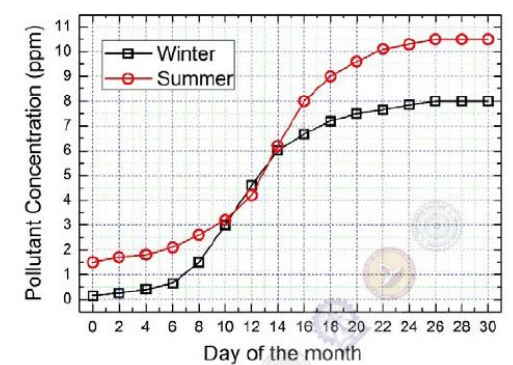
\includegraphics[width=0.5\columnwidth]{Figs/fig_14.png}
        \caption{Q.95.}
        \label{fig:placeholder_14}
    \end{figure}
    
    Consider the following statements based on the data shown above:\\
    $i$. Over the given months, the difference between the maximum and the minimum pollutant concentrations is the same in both winter and summer. \\
    $ii$. There are at least four days in the summer month such that the pollutant concentrations on those days are within $1$ ppm of the pollutant concentrations on the corresponding days in the winter month.
    
    Which one of the following options is correct? \hfill{\brak{\text{GATE GG 2017}}}
        \begin{enumerate}
            \begin{multicols}{4}
                \item Only $i$
                \item Only $ii$
                \item Both $i$ and $ii$
                \item Neither $i$ nor $ii$
            \end{multicols}
        \end{enumerate}
    

\centering\subsection*{END OF THE QUESTION PAPER}
\end{enumerate}
\end{document}

